\chapter{Ordinary Differential Equations}
% this section comes from MIT OCW ODE 18.035c Fall 2011 ed.
We will start by talking about \emph{first-order ordinary differential equations}\footnote{The following text comes from MIT OpenCourseWare notes on ODE 18.035c, Fall 2011 Edition},
that is, ordinary differential equations involving the first derivative.
They appear of the form:
\begin{equation}
  y'=f(x,y).
  \label{eq:fode}
\end{equation}

Let's take a look at the exponential function, which is absolutely invaluable in the study of differential equations.
It looks like
\[ x(t)=e^{at}. \]
\begin{figure}[H]
  \begin{center}
    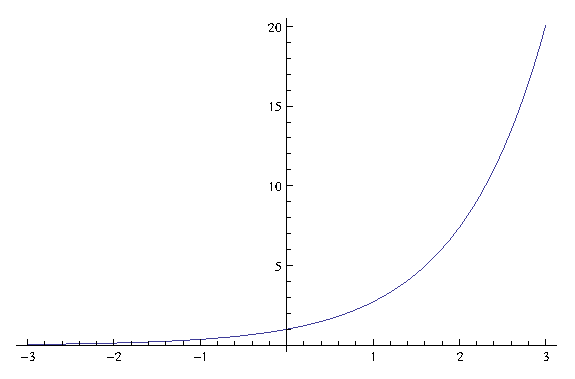
\includegraphics[width=2in]{continuous/ode/ept.eps}
  \end{center}
  \caption{A plot of $x(t)=e^t$.}
  \label{fig:plotept}
\end{figure}
This function has the following properties:
\begin{enumerate}
  \item $e^0 =1$.
  \item $e^{at+c} = e^c e^{at}$.
  \item $e^{at}$ is never zero.
  \item If $a>0$ then $\lim_{t\to 0} e^{at} = \infty$ and $\lim_{t\to -\infty} e^{at}=0$.
  \item If $a>0$ then $\lim_{t\to 0} e^at$ grows much faster than any polynomial.
    \begin{ex}
      $\lim_{t\to\infty} \frac{e^t}{t^3}=\infty$.
    \end{ex}
    \begin{ex}
      $\lim_{t\to\infty}te^{-t}=0.$
    \end{ex}
\end{enumerate}

In a function such as
\[ f(x)=3x^2+2x+1 \]
$x$ is the \textbf{independent variable}\index{independent variable}.
We can freely set it to any $x \in D$ and the function can then be computed.
When we give a name to the value of the function, as in
\[ y=3x^2 +2x +1 \]
or
\[y=f(x) \]
we say that $y$ is the \textbf{dependent variable}\index{dependent variable}.

We can have systems of equations with more than one dependent variable, as in
\[ x =t^2 -1 \]
or
\[ y=3e^t. \]
Here, the dependent variables $x$ and $y$ depend on the variable $t$.
We can have functions with multiple independent variables as well, such as
\[ x=st^2 -t -s. \]
Here, the independent variables are $s$ and $t$ and the dependent variable is $x$.

Or we can have more than one of each:
\[ x =st^2 -t -s \]
\[ y=3e^{t+s} \]
As an abuse of notation, we can use the dependent variable to denote the function, as in
\[ x=x(t)=t^2 -1.\]
Most of what we do will involve \textbf{ordinary differential equations}\index{ordinary differential equations} (ODEs).
These have only one dependent an one independent variable.

\textbf{Parameters}\index{parameters} are similar to variables.
They can take on different values within a set containing objects which are usually similar.
For example, in integrals we have equations like
\begin{equation}
  \int t^2 \ud t = \frac{t^3}{3}+c
  \label{eq:param1}
\end{equation}
so $c$ is a parameter. Each value of $c$ specifies an entire, similar antiderivative.

Sets are written ${t^3 /3 +c : \text{any number $c$}}$.
This means a set of functions $x=x(t)$ parameterized by $c$.
Sets can depend on more than one parameter, as in
\begin{equation}
  x(t)=c_1 e^{-t}+c_2 e^{-7t}
  \label{eq:param2}
\end{equation}
where $c_1$ and $c_2$ are arbitrary constants.

Equation \eqref{eq:param1} represents a $1$-parameter family of functions.
\eqref{eq:param2} represents a $2$-parameter family of functions.

We will write $\ud y / \ud x$, $y'$, or $D_y$ to mean \emph{the derivative of $y$ with respect to $x$.}
  Only the first way of writing this actually specifies the independent variable, which is $x$.
For second derivatives, we would write
\[ \frac{\ud ^2 y}{\ud x^2}= y''=D^2 y. \]

A differential equation expresses a relation between a function and its derivatives.
For example,
\[ \sqrt{x x^{5}}+\cos{(t)}e^{tx} + (x'' x' x )^6 = \sin{(5t)}. \]

The \textbf{order}\index{order} of a differential equation refers to the order of the highest derivative contained therein.

\textbf{Solving} an ODE means finding a function that satisfies the equation.
For many, this is hard or impossible.
It is easy, however, to check a proper solution.
\begin{ex}
  Verify $y(t)=e^{3t}$ is a solution for
  \[ y'=3y \]
  \begin{sol}
    \begin{align*}
      y&=3e^{3t} \\
      \ddx e^{3t} &=3e^{3t} \\
      3e^{3t} &= 3e^{3t}
    \end{align*}
  \end{sol}
\end{ex}
\begin{ex}
  Show that $y(t)=t^3$ is not a solution for \[y'=\frac{y}{t}.\]
  \begin{sol}
    \begin{align*}
      y'(t)&=3t^2 \\
      3t^2 &\neq \frac{t^3}{t}
    \end{align*}
  \end{sol}
\end{ex}
%\subsection{Parameterizing}
% terrible example
%\begin{ex}
%  Find all solutions for
%  \[ x''=2t.\]
%  \begin{sol}
%    \begin{align*}
%      \int 2t \ud t &= 2 \int t \ud t \\
%      &= t^2 + c_1 \\
%      \int (t+c_1) \ud t &= \frac{t^3}{3}+c_1 t +c_2
%    \end{align*}
%  \end{sol}
%\end{ex}
\begin{ex}
  Solve $x''=2t$ with the initial values $x(1)=1$, $x'(1)=2$.
  \begin{align*}
    x'&= t^2 +c_1 \\
    x'(t) &= t^2 + c_1 \\
    x'(1) &=2 \\
    2&= 1+c_1 \\
    c_1 &=1
  \end{align*}
  \begin{align*}
    1&=\frac{1}{3}+1+c_2 \\
    \frac{-1}{3} &= c_2
  \end{align*}
  \[ x(t) = \frac{t^3}{3}+t-\frac{1}{3} \]
\end{ex}

% in-class section
A common differential equation we will encounter is a \emph{freefall problem}\footnote{The following text comes from my Fall 2012 ordinary differential equations in-class lectures at Christopher Newport University.}.
Here's an example:

\begin{figure}[H]
  \begin{center}
    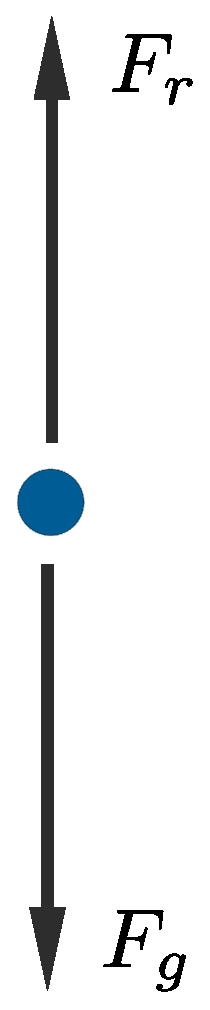
\includegraphics[width=1cm]{continuous/ode/freefall.eps}
  \end{center}
  \caption{A free-body diagram of an object in freefall.}
  \label{fig:freefall}
\end{figure}

Basic physics tells us that $\sum \vec F = m\vec a$,
where $m$ is the object's mass and $\vec{a}$ is the object's acceleration.
For our purposes, we will define $\vec F_g$ to be in the \emph{direction of increasing} $x$.
Based on these assumptions, we can state that
\[
  ma=\vec{F_g}+\vec{F_r}
  \]
Now, acceleration is the same as \emph{change in velocity,} so this is equivalent to
\[
  m\frac{\ud v}{\ud t}=mg - \gamma v
  \]
where $v$ is the object's velocity, $t$ is the time, $g$ is the acceleration of gravity near the surface of Earth, and $\gamma$ is the coefficient of friction for the air.

This is a \textbf{first-order linear ordinary differential equation}.

\begin{ex}
  Let's look at the differential equation
  \begin{equation}
    y'+3y=te^{-2t}
    \label{eq:prule}
  \end{equation}
  We solve this using a manipulation of the product rule for derivatives.
  It states that
  \begin{equation}
    \frac{\ud}{\ud t} f(x) g(x)= \frac{\ud f(x)}{\ud t} g(x) + \frac{\ud g(x)}{\ud t} f(x).
  \end{equation}
  We can rewrite Equation \eqref{eq:prule} to appear in this form using an \emph{integrating factor}\footnote{Define this.}.
  \[ \frac{\ud y}{\ud x}= t e^{-2t} \]
  If we take $y$ to equal $f(x)$ and the coefficient of $y$ in the second term to be $g(x)$, we realize that we must look for a $\mu (t) \ud t$ such that
  \begin{align*}
    \frac{\ud \mu}{\ud t} &= g(t) \mu(t) \\
    \mu (t) &= e^{\int 3 \ud t}\\
    &=e^{3t}
  \end{align*}
  to make the left side of Equation \eqref{eq:prule} satisfy the product rule.
  Note that we can ignore the arbitrary constant in $\mu (t)$ because it will eventually appear when we integrate both sides of \eqref{eq:prule}.

  Now, we multiply both sides of \eqref{eq:prule} by $\mu (t)$.
  \begin{align*}
    y'+3y &= te^{-2t} \\
    y' e^{3t} +3ye^{3t} &= te^{3t}+e^t \\
    \intertext{Use the product rule.}
    \frac{\ud y}{\ud t} \big[e^{3t}y\big] &=  te^{3t}+e^t \\
    \intertext{Integrate both sides.}
    e^{3t}y&=\frac{te^{3t}}{3}-\frac{e^{3t}}{9}+e^t+c\\
    y &=\frac{t}{3}-\frac{1}{9}+e^{-2t}+ce^{-3t}
  \end{align*}
\end{ex}
\begin{ex}
  \[y' +y = t e^{-t}+1\]
  \begin{sol}
    Multiply both sides by the integration factor $\mu (t) = e^t$.
    \begin{align*}
      y'e^t +ye^t &= t +e^t \\
      y e^t &= \frac{t^2}{2}+e^t+c \\
      y &= \frac{t}{2e}+1+\frac{c}{e^t}
    \end{align*}
  \end{sol}
\end{ex}
\begin{ex}
  \[y' -2y =3e^t\]
  \begin{sol}
    Multiply both sides by the integration factor $\mu(t) = e^{-2t}$.
    \begin{align*}
      y'e^{-2t} -2ye^{-2t} &= 3e^{-t} \\
      ye^{-2t} &= -3 e^{-t} +c \\
      y &= -3 e^t +ce^{2t}
    \end{align*}
  \end{sol}
\end{ex}
\begin{ex}
  \[ y' e^{t^2}+2tye^{t^2} = 2t \]
   \begin{sol}
    Multiply both sides by the integration factor $\mu(t) = e^{t^2}$.
    \begin{align*}
      y'e^{t^2}+2tye^{t^2} &= 2t \\
      y e^{t^2} &= t^2 +c \\
      y &= t^2 e^{-t^2}+ce^{-t^2}
    \end{align*}
  \end{sol}
\end{ex}
\begin{ex}
  \[y'e^{t/2}+\frac{ye^{t/2}}{2} = \frac{t}{2e^{t/2}} + \frac{e^{t/2}}{2} \]
  \begin{sol}
   Multiply both sides by the integration factor $\mu(t) = e^{t/2}$.
   \begin{align*}
     y'e^{t/2}+\frac{ye^{t/2}}{2} &= \frac{t}{2e^{t/2}} + \frac{e^{t/2}}{2} \\
     y e^{t/2} &= \int \left[ \frac{t}{2e^{t/2}} + \frac{e^{t/2}}{2} \right] \ud t \\
     \intertext{The indefinite integral $\int t e^{-t/2} \ud t$ is $-2t e^{-t/2}-4e^{-t/2}+c_1$, and the indefinite integral $\int e^{t/2} \ud t$ is $2e^{t/2}+c_2$.}
     ye^{t/2} &= \frac{2e^{t/2}-4e^{-t/2}-2te^{-t/2}}{2}+c \\
     ye^{t/2} &= e^{t/2} -2 e^{-t/2}-t e^{-t/2}+c \\
     y &= 1 -2e^{-t} -t e^{-t} + c e^{-t/2}
   \end{align*}
  \end{sol}
\end{ex}
\begin{ex}
  \[y' + y = 5 \sin {2t}\]
  \begin{sol}
   Multiply both sides by the integration factor $\mu (t) = e^t$.
   \begin{align*}
     y' e^t + ye^t &= 5 e^t \sin{2t} \\
     ye^t &= 5 \int e^t \sin{2t} \ud t \\
   \end{align*}
   Integrate $\int e^t \sin{2t} \ud t$. Use integration by parts with $u =\sin{2t}$ and $\ud v = e^t \ud t$.
   \begin{align*}
     \int e^t \sin{2t} \ud t &= e^t \sin{2t}-2 \int e^t \cos{2t} \ud t \\
     \intertext{Integrate by parts again, this time with $u = \cos{2t}$ and $\ud v=e^t \ud t$.}
     \int e^t \sin{2t} \ud t &= e^t \sin{2t}-2 \bigg[ e^t \cos{2t} + 2 \int e^t \sin{2t} \ud t \bigg] \\
     \int e^t \sin{2t} \ud t &= e^t \sin{2t}-2 e^t \cos{2t} -4 \int e^t \sin{2t} \ud t \\
     5\int e^t \sin{2t} \ud t &= e^t \sin{2t}-2 e^t \cos{2t}
   \end{align*}
   Substitute this into our differential equation.
   \begin{align*}
     ye^t &= 5 \int e^t \sin{2t} \ud t \\
     ye^t &= e^t \sin{2t} -2 e^t \cos^{2t} +c \\
     y &= \sin{2t}-2\cos{2t}+\frac{c}{e^t}
   \end{align*}
  \end{sol}
\end{ex}

These examples were all \textbf{first order linear equations}\index{first-order linear differential equation} of the standard form
\begin{equation}
  \frac{\ud y}{\ud t}+p(t)y=g(t),
  \label{eq:1ordlineq}
\end{equation}
where $p$ and $g$ are given functions of the independent variable $t$.\cite[p. 32]{boycede}

The \textbf{general first order equation}\index{general first-order differential equation} is
\begin{equation}
  \frac{\ud y}{\ud t}=ay+b.
\end{equation}
\cite[p. 42]{boycede}

If we can rewrite a first order equation in the form
\begin{equation}
  M(x)+N(y)\frac{\ud y}{\ud x}=0
  \label{eq:separableode}
\end{equation}
then it is \textbf{separable}\index{separable differential equation} because we can rewrite it
\begin{equation}
  M(x)\ud x+ N(y) \ud y=0
\end{equation}
then place the terms involving each variable on opposite sides of the equation.

If the right side of the equation $\ud y/\ud x=f(x,y)$ can be expressed as a function of the ratio $y/x$ only, then the equation is said to be \textbf{homogenous}\index{homogeneous differential equation}.
To solve these, introduce a new dependent variable $v$ such that $v=y/x$ or $y=xv(x)$.
Express $\ud y/\ud x$ in terms of $x$, $v$, and $\ud v/\ud x$.

An \textbf{autonomous} differential equation\index{autonomous differential equation} has the form
\begin{equation}
  \frac{\ud y}{\ud t}=f(y).
  \label{eq:autode}
\end{equation}

\begin{ex}
    Consider a lake of constant volume $V$ containing at time $t$ an amount $Q(t)$ of pollutant,
    evenly distributed throughout the lake with a concentration of $c(t)$, where $c(t)=Q(t)/V$.
    Assume that water containing a concentration $k$ of pollutant enters the lake at rate $r$,
    and that water leaves the lake at the same rate.
    Suppose that pollutants are also added to the lake at rate $P$.
    Note that the given assumptions neglect a number of factors that may, in some cases, be important--for example,
    the water added or lost by precipitation, absorption, or evaporation;
    the tendency of irregularities in the coastline to produce sheltered bays;
    and the fact that pollutants are not deposited evenly throughout the lake but (usually) at isolated points in its periphery.
    The results below must be interpreted in the light of the neglect of such factors as these. \cite[p. 63]{boycede}
    \begin{enumerate}
      \item[(a)]
        If at time $t=0$ the concentration of pollutant is $c_0$, find an expression for the concentration $c(t)$ at any time.
        What is the limiting concentration as $t\to\infty$?
        \begin{sol}
          We know that the rate of addition of pollutants is found using the equation
          \begin{equation*}
            \frac{\ud Q(t)}{\ud t} = \text{rate in} - \text{rate out}.
          \end{equation*}
          Our ``rate in'' constitutes both the rate at which polluted water is added to the lake,
          and the rate at which pollutants are directly added to the lake.
          Therefore,
          \[ \text{rate in}=kr+P. \]
          The ``rate out'' is found by multiplying the concentration of pollutant in the lake by the rate at which water leaves the lake.
          Therefore,
          \begin{align*}
            \text{rate out} &=r\, c(t),\\
            \intertext{which we could write as}
            \text{rate out}&= r \frac{Q(t)}{V}.
          \end{align*}

          Our rate of change for the pollutants then becomes
          \begin{equation}
            \frac{\ud Q(t)}{\ud t} = kr+P-r\frac{Q(t)}{V},
            \label{dqdt}
          \end{equation}
          Which we can rearrange in the form
          \begin{equation}
            \frac{\ud Q(t)}{\ud t}+\frac{r\, Q(t)}{V} = kr+P.
            \label{dqdtr}
          \end{equation}
          Multiplying \eref{dqdtr} by the integrating factor $\mu (t)=e^{rt/V}$ yields us
          \begin{equation}
            e^{rt/V}\frac{\ud Q(t)}{\ud t}+\frac{e^{rt/V}r}{V}Q(t) = e^{rt/V}kr+e^{rt/V}P.
            \label{dqif}
          \end{equation}
          Integrating both sides of \eref{dqif}, we obtain
          \begin{equation}
            e^{rt/V}Q(t) = \bigintssss \! \! \left[ e^{rt/V} kr + e^{rt/V}P\right] \ud t.
            \label{qint}
          \end{equation}
          Integrating the right side of \eref{qint} and solving for $Q(t)$, we obtain the general solution to \eref{dqdt}, that is
          \begin{equation}
            Q(t) =  kV+\frac{PV}{r}+a e^{-rt/V},
            \label{qtsol}
          \end{equation}
          where $a$ is an arbitrary constant.

          We can now find an expression for $c(t)$, which is given by
          \begin{equation}
            c(t) =\frac{Q(t)}{V}.
            \label{ct}
          \end{equation}
          Substituting \eref{qtsol} into \eref{ct}, we find that
          \begin{equation}
            c(t) = k + \frac{P}{r}+\frac{a e^{-rt/V}}{V}.
            \label{ct2}
          \end{equation}

          Using the initial value $c(0)=c_0$ and solving for $a$, we obtain
          \begin{equation}
            C=c_0 -\frac{P}{r}-k
            \label{csol}
          \end{equation}
          Substituting our value for $C$ back into \eref{ct2}, we find our solution to the initial value problem,
          \begin{equation}
            c(t)=k+\frac{P}{r}+e^{-rt/V}\left( c_0 - \frac{P}{r} -k\right).
            \label{ctbig}
          \end{equation}
          The factors of $e^{-rt/V}$
          will become negligible because $e^{-rt/V}$ approaches zero as $t\to\infty$.
          Thus, the limiting concentration of pollutants in the lake is given by
          \begin{equation}
            \lim_{t\to\infty} c(t) = k+\frac{P}{r}.
            \label{limc}
          \end{equation}
       \end{sol}
      \item[(b)]
        If the addition of pollutants to the lake is terminated ($k=0$ and $P=0$ for $t>0$),
        determine the time interval $T$ that must elapse before the concentration of pollutants is reduced to $50\%$ of its original value;
        to $10\%$ of its original value.

        \begin{sol}
          Since $k=0$ and $P=0$, we can neglect the first and last two terms of \eref{ctbig}.
          To find the time interval $T$ where the pollutants have reached a given fraction, which we will call $\alpha$, of their original value,
          we must remember that $c_0$ is the original concentration and find the value for $t$ where
          \begin{equation}
            c(t) = \frac{c_0}{\alpha}.
            \label{halfc}
          \end{equation}
          To achieve this, we replace $c(t)$ in \eref{halfc} with $c_0/\alpha$ and replace the variable $t$ with the variable for our time interval, $T$.
          This shows that
          \begin{equation}
            \frac{c_0}{\alpha}=c_0 e^{-rT/V}.
            \label{halfceq}
          \end{equation}
          We divide by $c_0$ and take the natural logarithm of both sides, finding that
          \begin{equation}
            -\frac{rT}{V}=\ln{\alpha},
            \label{Tnlog}
          \end{equation}
          provided that $\alpha > 0$.

          To solve for $T$, we multiply both sides of this equation by $-V/r$, which gives us the value of $T$,
          \begin{equation}
            T = \frac{-V\ln{\alpha}}{r}.
            \label{tsol}
          \end{equation}
          For the time interval that must elapse before the concentration of pollutants is reduced to $50\%$ of its original value, $\alpha=1/2$ and
          \begin{equation}
            T=\frac{V\ln2}{r}.
          \end{equation}
          Likewise, to find the time interval that must elapse before the concentration of pollutants is reduced to $10\%$ of its original value, $\alpha=1/10$ and
          \begin{equation}
            T=\frac{V \ln{10}}{r}.
          \end{equation}
        \end{sol}
      \item[(c)]
        Table \ref{tab:volflow} contains data for several of the Great Lakes.
        Using these data, determine from part (b) the time $T$ necessary to reduce the contamination of each of these lakes
        to $10\%$ of its original value.
        \begin{table}[H]
          \begin{center}
            \begin{tabular}{ccc}
              \hline
              Lake & $V(\text{km}^3\times 10^3)$ & $r(\text{km}^3/\text{year})$ \\ \hline
              Superior & 12.2 & 65.2 \\
              Michigan & 4.9 & 158 \\
              Erie & 0.46 & 175 \\
              Ontario & 1.6 & 209 \\ \hline
            \end{tabular}
            \caption{Volume and Flow Data for the Great Lakes}
          \end{center}
          \label{tab:volflow}
        \end{table}
        \begin{sol}
          For Lake Superior,
          \begin{align*}
            T&=\frac{\left(12.2\, \text{km}^3 \times 10^3\right) \ln{10}}{65.2\, \text{km}^3/\text{year}} \\
            &=430.852\; \text{years}.
          \end{align*}

          For Lake Michigan,
          \begin{align*}
            T&=\frac{\left(4.9\, \text{km}^3 \times 10^3\right) \ln{10}}{158\, \text{km}^3/\text{year}} \\
            &=71.4093\; \text{years}.
          \end{align*}

          For Lake Erie,
          \begin{align*}
            T&=\frac{\left(0.46 \, \text{km}^3 \times 10^3\right) \ln{10}}{175\, \text{km}^3/\text{year}} \\
            &=6.05251\; \text{years}.
          \end{align*}

          For Lake Ontario,
          \begin{align*}
            T&=\frac{\left(1.6\, \text{km}^3 \times 10^3\right) \ln{10}}{209\, \text{km}^3/\text{year}} \\
            &=17.6274\; \text{years}.
          \end{align*}
        \end{sol}
    \end{enumerate}
\end{ex}
\begin{ex}
  Solve \[\frac{\ud y}{\ud t}=3(1-\frac{y}{5})y. \]
  \begin{sol}\footnote{Honestly, I have no idea if this is correct or not. I haven't checked it at all.}
    \begin{align*}
      \frac{\frac{\ud y}{\ud t}}{y(1-y/5)}&=3 \\
      \frac{\ud y}{\ud t}\left[\frac{1}{y}+\frac{1}{5-y}\right]&=3 \\
      \log y - \log{(5-y)}&=3t+c_1 \\
      y^2&=e^{3x}+c-5 \\
      y= \sqrt{e^{3x}+c-5}
    \end{align*}
  \end{sol}
\end{ex}
